\documentclass[1p,times]{elsarticle}

\usepackage[utf8]{inputenc}
\usepackage[vietnamese]{babel}
\usepackage[T1,T5]{fontenc}
\usepackage{amsmath,amssymb,amsfonts} 
\usepackage{graphicx} 
\usepackage{float}
\usepackage{algorithm}
\usepackage{algpseudocode}
\usepackage{multirow} 
\usepackage{booktabs} 
\usepackage{fancyhdr}
\usepackage{placeins}
\usepackage{hyperref}
\hypersetup{
    colorlinks=true,
    linkcolor=blue,
    citecolor=blue,
    urlcolor=blue
}

\pagestyle{fancy}
\fancyhf{} 
\fancyhead[LE,RO]{\textbf{\thepage}} 
\fancyhead[C]{\small Khảo Sát \& Đánh Giá: Chuỗi Bộ Phân Loại và Học Sâu Bằng Chứng trong Phân Loại Đa Nhãn} 
\renewcommand{\headrulewidth}{0.5pt} 

% Định nghĩa tên tạp chí
\journal{Expert Systems with Applications}

\begin{document}

\begin{frontmatter}

\title{Khảo Sát Toàn Diện và Đánh Giá Thực Nghiệm Về Họ Chuỗi Bộ Phân Loại Trong Phân Loại Đa Nhãn Mất Cân Bằng: Từ Mô Hình Cổ Điển Đến Học Sâu Bằng Chứng (EDL-ECC)}

\author{Nhóm Nghiên Cứu Machine Learning}
\address{Phòng Thí Nghiệm Trí Tuệ Nhân Tạo và Khoa Học Dữ Liệu}

\begin{abstract}
Phân loại đa nhãn (Multi-Label Classification — MLC) đóng vai trò then chốt trong nhiều lĩnh vực công nghệ cao như chẩn đoán y sinh, phân loại văn bản và thị giác máy tính. Tuy nhiên, bài toán này đối mặt với hai rào cản mang tính cốt lõi: sự phụ thuộc phức tạp giữa các nhãn và tình trạng mất cân bằng dữ liệu cực đoan. Trong số các họ phương pháp tiếp cận, Chuỗi Bộ Phân Loại (Classifier Chains — CC) và biến thể kết hợp (Ensemble Classifier Chains — ECC) là những giải pháp kinh điển để nắm bắt tương quan nhãn nhưng lại vướng phải hiện tượng lan truyền sai số (error propagation) dọc theo chuỗi. 

Bài báo này đóng vai trò một công trình khảo sát toàn diện (systematic survey) và đánh giá thực nghiệm (benchmark study) về họ mô hình chuỗi phân loại trong môi trường dữ liệu mất cân bằng. Chúng tôi phân tích có hệ thống cấu trúc phân loại học (taxonomy) của MLC, làm sáng tỏ bản chất toán học của hiện tượng lan truyền sai số, và chỉ ra khiếm khuyết chết người của các bộ phân loại cơ sở dựa trên hàm Softmax/Sigmoid: sự tự tin thái quá (overconfidence) khi gặp nhãn thiểu số. Từ đó, chúng tôi khảo sát sâu kiến trúc lai EDL-ECC (Evidential Ensemble Classifier Chains), giải pháp tích hợp Học Sâu Bằng Chứng (Evidential Deep Learning — EDL) dựa trên phân phối Dirichlet vào khung ECC. Thông qua cơ chế truyền đặc trưng nhận thức độ bất định (Uncertainty-Aware Feature Propagation), EDL-ECC định lượng tường minh độ bất định nhận thức (epistemic uncertainty) để chủ động dập tắt các tín hiệu sai lệch lan truyền. Thử nghiệm kiểm chứng chéo 5-Fold trên 9 tập dữ liệu chuẩn đối chứng đa tầng giữa 4 mô hình đại diện (BR, CC, ECC và EDL-ECC) cùng các kiểm định phi tham số Friedman ($p < 0.001$) và Wilcoxon ($p = 9.79 \times 10^{-9}$) khẳng định: Ensemble thuần túy (ECC) không thể cứu vãn lan truyền sai số trên dữ liệu mất cân bằng nặng, trong khi EDL-ECC tạo ra bước nhảy vọt Macro-F1 (tăng tới $+37.2\%$ trên HumanPseAAC). Cuối cùng, bài báo thảo luận sâu sắc về các ngộ nhận lý thuyết, hiện tượng đánh đổi độ chính xác (accuracy paradox), các hạn chế nội tại của phương pháp và gợi mở các hướng nghiên cứu tiềm năng trong tương lai.
\end{abstract}

\begin{keyword}
Phân loại đa nhãn \sep Chuỗi bộ phân loại \sep Học sâu bằng chứng \sep Độ bất định nhận thức \sep Dữ liệu mất cân bằng \sep Khảo sát toàn cảnh
\end{keyword}

\end{frontmatter}

% ==========================================
% 1. GIỚI THIỆU
% ==========================================
\section{Giới Thiệu và Động Lực Khảo Sát}
\label{sec:intro}

Trong kỷ nguyên Trí tuệ Nhân tạo hiện đại, bài toán Học Đa Nhãn (Multi-Label Learning — MLL) và cụ thể là Phân Loại Đa Nhãn (Multi-Label Classification — MLC) \citep{tsoumakas2007multi, zhang2014review, gibaja2015tutorial} đã trở thành một nhánh nghiên cứu nền tảng, mở rộng từ bài toán phân loại đơn nhãn truyền thống. Trong MLC, mỗi mẫu dữ liệu đầu vào $\mathbf{x} \in \mathbb{R}^D$ không chỉ thuộc về một lớp duy nhất mà được liên kết đồng thời với một tập con các nhãn mục tiêu $\mathbf{y} \in \{0, 1\}^K$. Không gian đầu ra của bài toán vì thế bùng nổ theo cấp số nhân ($2^K$ tổ hợp khả dĩ), phản ánh bản chất ngữ nghĩa phong phú nhưng vô cùng phức tạp của thế giới thực. Ví dụ tiêu biểu bao gồm: trong y học, một ảnh X-quang phổi có thể chứa đồng thời dấu hiệu tràn dịch, viêm phổi và xơ hóa \citep{wang2017chestx}; trong proteomics, một chuỗi protein có thể cùng lúc sở hữu nhiều chức năng sinh học hoặc khu trú tại nhiều vị trí dưới tế bào \citep{chou2011pseacc}; trong thị giác máy tính, một bức ảnh phong cảnh thường đồng thời chứa các nhãn \textit{núi}, \textit{rừng}, và \textit{bầu trời} \citep{boutell2004learning}.

Mặc dù có tiềm năng ứng dụng rộng lớn, việc xây dựng các hệ thống MLC có độ tin cậy cao đang vấp phải ba thách thức cốt lõi chưa có lời giải triệt để:
\begin{enumerate}
    \item \textbf{Thách thức về Tương quan Nhãn (Label Correlation Dilemma):} Các nhãn trong thực tế hiếm khi độc lập thống kê mà ràng buộc chặt chẽ thông qua các quan hệ đồng xuất hiện, loại trừ tương hỗ hoặc phân cấp ngữ nghĩa. Việc mô hình hóa tương quan bậc cao đòi hỏi chi phí tính toán bùng nổ, tạo ra sự đánh đổi khắc nghiệt giữa độ chính xác và tính khả thi thuật toán.
    \item \textbf{Thách thức Mất Cân Bằng Dữ Liệu Kép (Dual Imbalance Problem):} Dữ liệu đa nhãn đồng thời chịu tác động của mất cân bằng nội nhãn (số lượng mẫu âm tính vượt trội mẫu dương tính ở hầu hết các nhãn) và mất cân bằng liên nhãn (một số ít nhãn phổ biến chiếm ưu thế hoàn toàn so với các nhãn hiếm gặp) \citep{charte2015addressing}. Các mô hình học máy thông thường có xu hướng bị chệch về lớp đa số, dẫn đến sự suy giảm nghiêm trọng trên các nhãn thiểu số.
    \item \textbf{Thách thức về Tự Tin Thái Quá và Thiếu Nhận Thức Độ Bất Định (Overconfidence and Epistemic Uncertainty):} Trong các hệ thống chuyên gia hỗ trợ ra quyết định rủi ro cao (chẩn đoán bệnh, phát hiện gian lận tài chính, giám sát môi trường), việc một mạng nơ-ron đưa ra phán đoán sai lệch nhưng với mức độ tự tin gần như tuyệt đối (overconfidence) là một hiểm họa khôn lường \citep{guo2017calibration, hullermeier2021aleatoric}.
\end{enumerate}

Để nắm bắt tương quan nhãn, họ phương pháp Chuỗi Bộ Phân Loại (Classifier Chains — CC) \citep{read2011classifier} đã trở thành một cột mốc quan trọng nhờ khả năng truyền dự đoán nhãn trước làm đặc trưng bổ sung cho nhãn sau. Nhằm khắc phục tính nhạy cảm với thứ tự nhãn của CC, kiến trúc Chuỗi Kết Hợp (Ensemble Classifier Chains — ECC) ra đời, sử dụng cơ chế trung bình hóa nhiều chuỗi ngẫu nhiên. Tuy nhiên, khi đối mặt với dữ liệu mất cân bằng, cả CC và ECC đều bộc lộ một lỗ hổng chí mạng: \textit{hiện tượng lan truyền sai số phá hủy (destructive error propagation)}. Khi một bộ phân loại ở đầu chuỗi đưa ra dự đoán sai lệch trên nhãn thiểu số nhưng lại mang độ tự tin cao giả tạo do hàm Softmax/Sigmoid sinh ra, sai số này sẽ làm "nhiễm độc" toàn bộ dòng thông tin truyền dọc theo chuỗi.

Gần đây, sự xuất hiện của Học Sâu Bằng Chứng (Evidential Deep Learning — EDL) \citep{sensoy2018evidential} dựa trên nền tảng Logic Chủ Quan (Subjective Logic) \citep{josang2016subjective} và phân phối Dirichlet đã mở ra hướng đi đột phá trong việc lượng hóa tường minh độ bất định nhận thức (epistemic uncertainty). Sự kết hợp giữa EDL và ECC (tạo nên kiến trúc EDL-ECC) hứa hẹn cung cấp một cơ chế điều tiết tự động dập tắt sai số lan truyền.

Tuy nhiên, trong các công bố hiện có, còn tồn tại sự thiếu vắng các nghiên cứu khảo sát có hệ thống phân tích sâu sắc mối liên kết hiệp đồng (synergy) giữa EDL và ECC, cũng như thiếu vắng các thử nghiệm đối chứng toàn diện (ablation benchmark) phân định rõ vai trò độc lập của từng thành phần. Bài báo này được xây dựng nhằm lấp đầy khoảng trống học thuật đó với bốn đóng góp chính:
\begin{itemize}
    \item Cung cấp một khung phân loại học (taxonomy) toàn diện về các trường phái tiếp cận trong MLC, định vị chính xác vị trí của họ mô hình chuỗi phân loại và các phương pháp nhận thức độ bất định.
    \item Phân tích tường minh cơ chế toán học của hiện tượng lan truyền sai số, chứng minh bản chất gây hại của hiện tượng tự tin thái quá trong hàm Softmax/Sigmoid, và giải trình sự kết hợp hiệp đồng $1 + 1 > 2$ giữa EDL và ECC.
    \item Thiết lập một benchmark thực nghiệm đa tầng nghiêm ngặt trên 9 tập dữ liệu chuẩn thuộc nhiều lĩnh vực, so sánh đầy đủ 4 mô hình (BR, CC, ECC, EDL-ECC) trên 5 độ đo tiêu chuẩn, đi kèm kiểm định thống kê phi tham số.
    \item Thảo luận khách quan về các ngộ nhận lý thuyết, hiện tượng đánh đổi nghịch lý độ chính xác (accuracy paradox), chỉ ra các hạn chế cố hữu của phương pháp và vạch ra các hướng nghiên cứu mở.
\end{itemize}

% ==========================================
% 2. PHÂN LOẠI HỌC TOÀN CẢNH TRONG MLC
% ==========================================
\section{Hệ Thống Phân Loại Học Toàn Cảnh Trong Phân Loại Đa Nhãn}
\label{sec:taxonomy}

\subsection{Hình Thức Hóa Toán Học Bài Toán MLC}
Cho $\mathcal{X} = \mathbb{R}^D$ là không gian đặc trưng đầu vào và $\mathcal{L} = \{l_1, l_2, \dots, l_K\}$ là tập hữu hạn gồm $K$ nhãn phân biệt. Tập dữ liệu huấn luyện được cho bởi $\mathcal{D} = \{(\mathbf{x}_i, \mathbf{y}_i)\}_{i=1}^N$, trong đó $\mathbf{x}_i \in \mathcal{X}$ và vector nhị phân $\mathbf{y}_i = [y_{i,1}, y_{i,2}, \dots, y_{i,K}]^\top \in \mathcal{Y} = \{0, 1\}^K$. Giá trị $y_{i,j} = 1$ biểu thị mẫu $\mathbf{x}_i$ mang nhãn $l_j$, ngược lại $y_{i,j} = 0$. Mục tiêu của MLC là học hàm ánh xạ:
\begin{equation}
    f: \mathcal{X} \to \{0, 1\}^K \quad \text{hoặc} \quad h: \mathcal{X} \to [0, 1]^K
\end{equation}
trong đó $h(\mathbf{x})$ xuất ra vector xác suất dự đoán cho từng nhãn.

Để đặc trưng hóa độ phức tạp của tập dữ liệu đa nhãn, văn hiến chuẩn mực \citep{tsoumakas2007multi, zhang2014review} sử dụng hai chỉ số thống kê nền tảng:
\begin{itemize}
    \item \textbf{Lực lượng nhãn (Label Cardinality — $\text{LCar}$):} Số lượng nhãn dương tính trung bình trên mỗi mẫu dữ liệu:
    \begin{equation}
        \text{LCar}(\mathcal{D}) = \frac{1}{N} \sum_{i=1}^N \sum_{j=1}^K y_{i,j}
    \end{equation}
    \item \textbf{Mật độ nhãn (Label Density — $\text{LDen}$):} Tỷ lệ nhãn dương tính trung bình chuẩn hóa theo tổng số nhãn $K$:
    \begin{equation}
        \text{LDen}(\mathcal{D}) = \frac{\text{LCar}(\mathcal{D})}{K} = \frac{1}{N \cdot K} \sum_{i=1}^N \sum_{j=1}^K y_{i,j}
    \end{equation}
\end{itemize}

\subsection{Cấu Trúc Phân Loại Học (Taxonomy)}
Dựa trên cách thức tiếp cận bài toán và mức độ khai thác tương quan nhãn, các phương pháp học đa nhãn trong văn hiến được phân chia thành ba trường phái chính, như được hệ thống hóa trong Bảng \ref{tab:taxonomy_comparison}.

\begin{table}[htbp]
\centering
\caption{Hệ thống phân loại học các phương pháp trong Học Đa Nhãn (MLC).}
\label{tab:taxonomy_comparison}
\small
\begin{tabular*}{\textwidth}{@{\extracolsep{\fill}}lp{3.2cm}p{3.8cm}p{3.6cm}}
\toprule
\textbf{Trường phái} & \textbf{Phương pháp tiêu biểu} & \textbf{Cơ chế tương quan nhãn} & \textbf{Hạn chế chính} \\
\midrule
\textbf{1. Biến đổi bài toán} & Binary Relevance (BR) & Bậc 0 (Giả định độc lập hoàn toàn) & Bỏ qua tương quan nhãn. \\
\textit{(Problem} & Classifier Chains (CC) & Bậc 1 (Chuỗi tuần tự) & Lan truyền sai số; nhạy cảm thứ tự. \\
\textit{Transformation)} & Ensemble CC (ECC) & Bậc cao (Trung bình hóa ngẫu nhiên) & Tốn kém tính toán; overconfidence. \\
 & Label Powerset (LP) & Toàn cục (Gộp $2^K$ tổ hợp thành đa lớp) & Bùng nổ không gian lớp; thưa dữ liệu. \\
 & RAkEL & Bậc cao cục bộ (Tập hợp tổ hợp ngẫu nhiên) & Chi phí tính toán tăng khi $K$ lớn. \\
\midrule
\textbf{2. Thích ứng thuật toán} & ML-kNN & Tương quan qua láng giềng k-NN & Nhạy cảm với nhiễu đặc trưng. \\
\textit{(Algorithm} & ML-DT (C4.5 đa nhãn) & Tương quan thông qua hàm Entropy đa nhãn & Khó bắt phụ thuộc phi tuyến phức tạp. \\
\textit{Adaptation)} & Rank-SVM & Cặp nhãn (Pairwise ranking loss) & Độ phức tạp bậc hai theo số nhãn. \\
\midrule
\textbf{3. Học sâu \&} & Deep MLC (BCE / ASL) & Tương quan qua biểu diễn ẩn chung & Dễ overconfident; uncalibrated. \\
\textbf{Nhận thức độ bất định} & Bayesian Neural Net (BNN) & Ước lượng hậu nghiệm qua MC-Dropout & Chi phí lấy mẫu lớn khi suy luận. \\
\textit{(Uncertainty-Aware)} & \textbf{EDL-ECC (Đề xuất)} & \textbf{Bậc cao + Nhận thức độ bất định} & \textbf{Huấn luyện $M \times K$ mô hình MLP.} \\
\bottomrule
\end{tabular*}
\end{table}

% ==========================================
% 3. PHÂN TÍCH CHUYÊN SÂU HỌ CHUỖI PHÂN LOẠI
% ==========================================
\section{Phân Tích Chuyên Sâu Họ Chuỗi Phân Loại và Bản Chất Lan Truyền Sai Số}
\label{sec:chain_family}

\subsection{Cơ Sở Toán Học Của Quy Tắc Nhân Chuỗi Xác Suất}
Xét bài toán ước lượng phân phối đồng thời của vector nhãn $\mathbf{y}$ có điều kiện trên đầu vào $\mathbf{x}$. Dựa trên quy tắc nhân xác suất điều kiện (probabilistic chain rule), phân phối đồng thời được khai triển chính xác:
\begin{equation}
    P(y_1, y_2, \dots, y_K \mid \mathbf{x}) = \prod_{j=1}^K P(y_j \mid \mathbf{x}, y_1, \dots, y_{j-1})
    \label{eq:chain_rule}
\end{equation}

Mô hình Classifier Chains (CC) \citep{read2011classifier} hiện thực hóa công thức (\ref{eq:chain_rule}) bằng cách huấn luyện $K$ bộ phân loại nhị phân tuần tự. Bộ phân loại thứ $j$ được huấn luyện trên không gian đặc trưng mở rộng:
\begin{equation}
    \mathbf{x}^{(j)} = [\mathbf{x}^\top, y_1, \dots, y_{j-1}]^\top \in \mathbb{R}^{D + j - 1}
\end{equation}
Trong giai đoạn suy luận, do không biết trước giá trị nhãn thực tế của các bước trước, CC buộc phải thay thế $y_1, \dots, y_{j-1}$ bằng các giá trị dự đoán nhị phân cứng $\hat{y}_1, \dots, \hat{y}_{j-1}$:
\begin{equation}
    \hat{y}_j = \arg\max_{c \in \{0, 1\}} \hat{P}(y_j = c \mid \mathbf{x}, \hat{y}_1, \dots, \hat{y}_{j-1})
\end{equation}

\subsection{Bản Chất Hiện Tượng Lan Truyền Sai Số (Error Propagation Mechanism)}
Mặc dù CC mô phỏng quy tắc nhân xác suất rất tự nhiên, mô hình này chịu một khiếm khuyết cơ bản giữa huấn luyện và suy luận (\textit{exposure bias} hoặc \textit{train-test distribution discrepancy}):
\begin{itemize}
    \item \textbf{Trong lúc huấn luyện:} Bộ phân loại thứ $j$ luôn nhận được đặc trưng nhãn trước hoàn hảo từ nhãn thực tế $y_1, \dots, y_{j-1}$.
    \item \textbf{Trong lúc suy luận:} Bộ phân loại thứ $j$ phải nhận các dự đoán có sai số $\hat{y}_1, \dots, \hat{y}_{j-1}$.
\end{itemize}

Nếu tồn tại một mắt xích thứ $k$ ở đầu chuỗi bị phân loại sai ($\hat{y}_k \neq y_k$), một vector đặc trưng bị "nhiễm độc" sẽ được truyền sang mắt xích $k+1$. Giả sử xác suất phân loại đúng độc lập điều kiện tại mỗi mắt xích là $1 - \epsilon$. Xác suất để toàn bộ chuỗi đưa ra một vector nhãn chính xác tuyệt đối giảm nhanh theo hàm số mũ:
\begin{equation}
    P(\hat{\mathbf{y}} = \mathbf{y} \mid \mathbf{x}) = \prod_{j=1}^K (1 - \epsilon_j) \le (1 - \epsilon_{\min})^K
\end{equation}
Đặc biệt trên các tập dữ liệu mất cân bằng nặng, các nhãn thiểu số có tỷ lệ lỗi $\epsilon$ rất lớn. Khi một nhãn hiếm bị đặt ở đầu chuỗi, lỗi sai ngay lập tức kích hoạt hiệu ứng domino làm sụp đổ toàn bộ chuỗi phân loại phía sau.

\subsection{So Sánh Đa Tầng: BR, CC, ECC và EDL-ECC}
Nhằm làm rõ sự tiến hóa về mặt giải thuật và nguyên lý hoạt động trước khi đi vào phân tích số liệu thực nghiệm, Bảng \ref{tab:multi_tier_comparison} đối chiếu toàn diện 4 mô hình theo 6 tiêu chí kỹ thuật then chốt.

\begin{table}[htbp]
\centering
\caption{So sánh đa tầng cơ chế hoạt động giữa BR, CC, ECC và EDL-ECC.}
\label{tab:multi_tier_comparison}
\small
\begin{tabular*}{\textwidth}{@{\extracolsep{\fill}}lp{2.6cm}p{2.8cm}p{3.2cm}p{3.2cm}}
\toprule
\textbf{Tiêu chí} & \textbf{Binary Relevance (BR)} & \textbf{Classifier Chains (CC)} & \textbf{Ensemble CC (ECC)} & \textbf{EDL-ECC (Đề xuất)} \\
\midrule
\textbf{Mô hình hóa} & Không (Giả định độc & Bậc 1 tuần tự & Bậc cao trung bình hóa & Bậc cao có nhận thức \\
\textbf{tương quan} & lập hoàn toàn). & $(\mathbf{x}, \hat{y}_1, \dots, \hat{y}_{j-1})$. & qua $M$ chuỗi ngẫu nhiên. & độ tin cậy $[\hat{p}, u]^\top$. \\
\midrule
\textbf{Lan truyền} & Không có & Rất nghiêm trọng & Giảm nhẹ nhờ trung & Bị dập tắt chủ động \\
\textbf{sai số} & (Do dự đoán độc lập). & (Hiệu ứng domino). & bình hóa đa chuỗi. & khi $u \approx 1$. \\
\midrule
\textbf{Nhạy cảm} & Không áp dụng. & Rất cao & Rất thấp (Trung bình & Rất thấp (Ensemble + \\
\textbf{thứ tự nhãn} & & (Bài toán NP-hard). & trên $M$ hoán vị). & triệt tiêu tín hiệu lỗi). \\
\midrule
\textbf{Tín hiệu truyền} & Không có. & Nhãn cứng: & Nhãn cứng hoặc & Vector hai chiều: \\
\textbf{dọc chuỗi} & & $\hat{y} \in \{0, 1\}$. & xác suất: $p \in [0, 1]$. & $[\hat{p}, u]^\top \in [0, 1]^2$. \\
\midrule
\textbf{Hành vi trên} & Kém (Thiên vị nhãn & Rất kém (Sai sót đầu & Trung bình (Vẫn chịu & Xuất sắc (Dirichlet \\
\textbf{mất cân bằng} & đa số, bỏ qua hiếm). & chuỗi bị khuếch đại). & ảnh hưởng overconfidence). & dập overconfidence). \\
\midrule
\textbf{Khả năng} & Không thể & Không thể & Không thể & Có thể (Từ chối tự động \\
\textbf{từ chối an toàn} & (Chỉ có xác suất giả). & (Không có uncertainty). & (Chỉ có xác suất điểm). & khi $\bar{U} \ge \tau_u$). \\
\bottomrule
\end{tabular*}
\end{table}

\subsection{Tầm Quan Trọng Độc Lập và Tính Hiệp Đồng (Synergy) Giữa EDL và ECC}
Một câu hỏi lý thuyết cốt lõi được đặt ra: \textit{Tại sao cần kết hợp cả EDL và ECC mà không sử dụng riêng lẻ từng thành phần?}

\subsubsection{EDL giải quyết gì mà các mô hình trước đây chưa đạt được?}
Các mạng nơ-ron truyền thống sử dụng hàm Softmax hoặc Sigmoid đều đưa ra các \textit{ước lượng điểm (point estimates)}. Bản chất toán học của phép chuẩn hóa này ép buộc tổng xác suất bằng 1, dẫn đến hiện tượng tự tin thái quá (overconfidence) \citep{guo2017calibration}. Ngay cả khi mẫu dữ liệu rơi vào vùng không gian thưa thớt hoặc thuộc nhãn thiểu số chưa có đủ dữ liệu học, mạng vẫn gán xác suất cao cho một lớp nào đó. 

EDL giải quyết tận gốc rào cản này bằng cách mô hình hóa đầu ra dưới dạng phân phối Dirichlet thông qua Logic Chủ Quan (Subjective Logic) \citep{josang2016subjective, sensoy2018evidential}. EDL phân rã rành mạch giữa \textit{độ bất định ngẫu nhiên (aleatoric uncertainty)} và \textit{độ bất định nhận thức (epistemic uncertainty)}. Khi thiếu dữ liệu, mạng không sinh bằng chứng ($e \approx 0 \Rightarrow S \approx 2$), kéo theo độ bất định nhận thức đạt mức tối đa ($u \to 1$). Khả năng chủ động nói \textbf{"Tôi không chắc chắn"} chính là bước đột phá nền tảng của EDL.

\subsubsection{ECC giải quyết gì mà CC đơn lẻ chưa đạt được?}
Mô hình CC chuẩn phụ thuộc sinh tử vào thứ tự sắp xếp các nhãn $\mathcal{O} = (\pi_1, \dots, \pi_K)$. Việc tìm kiếm thứ tự nhãn toàn cục tối ưu là một bài toán NP-khó ($K!$ hoán vị khả dĩ). ECC giải quyết bài toán này bằng cách sinh ra $M$ chuỗi với thứ tự ngẫu nhiên, thực hiện suy luận song song và lấy trung bình cộng xác suất. Cơ chế ensemble giúp giảm thiểu phương sai (variance reduction) và phân tán rủi ro khi chọn nhầm thứ tự xấu.

\subsubsection{Sự kết hợp hiệp đồng: 1 + 1 > 2}
\begin{itemize}
    \item \textbf{Nếu chỉ có EDL đứng một mình (EDL-BR):} Ta thu được các bộ phân loại nhị phân biết lượng hóa độ bất định, nhưng mô hình hoàn toàn mất đi khả năng khai thác mối quan hệ tương hỗ giữa các nhãn.
    \item \textbf{Nếu chỉ có ECC đứng một mình:} Ta có cấu trúc chuỗi nắm bắt tương quan, nhưng dòng chảy thông tin bị ô nhiễm nặng nề bởi các phán đoán sai nhưng tự tin của các base classifier truyền thống.
    \item \textbf{Khi tích hợp EDL vào ECC (EDL-ECC):} ECC cung cấp \textit{hạ tầng đồ thị lan truyền thông tin} (Information Highway), còn EDL đóng vai trò \textit{bộ điều tiết chất lượng tín hiệu} (Uncertainty-Aware Signal Regulator). Nhờ đó, EDL dập tắt sai số lan truyền trên từng mắt xích, bảo vệ vững chắc cấu trúc ensemble.
\end{itemize}

% ==========================================
% 4. NỀN TẢNG LÝ THUYẾT EDL VÀ KIẾN TRÚC EDL-ECC
% ==========================================
\section{Nền Tảng Lý Thuyết Học Sâu Bằng Chứng và Kiến Trúc EDL-ECC}
\label{sec:method}

\subsection{Logic Chủ Quan và Phân Phối Dirichlet}
Trong khung Logic Chủ Quan cho bài toán nhị phân \citep{josang2016subjective}, trạng thái niềm tin đối với nhãn $j$ được mô hình hóa bằng bộ ba: lượng niềm tin (belief) $b_j$, lượng nghi ngờ (disbelief) $d_j$, và độ bất định nhận thức (uncertainty) $u_j$, thỏa mãn điều kiện tiên quyết:
\begin{equation}
    b_j + d_j + u_j = 1, \quad b_j, d_j, u_j \ge 0
\end{equation}

Các đại lượng này được liên kết chặt chẽ với vector bằng chứng $\mathbf{e}_j = [e_{j,0}, e_{j,1}]^\top \ge 0$ thông qua tham số phân phối Beta (trường hợp nhị phân của phân phối Dirichlet) $\boldsymbol{\alpha}_j = [\alpha_{j,0}, \alpha_{j,1}]^\top = [e_{j,0} + 1, e_{j,1} + 1]^\top$:
\begin{equation}
    b_j = \frac{e_{j,1}}{S_j}, \quad d_j = \frac{e_{j,0}}{S_j}, \quad u_j = \frac{2}{S_j}
\end{equation}
trong đó $S_j = \alpha_{j,0} + \alpha_{j,1} = e_{j,0} + e_{j,1} + 2$ là tổng cường độ Dirichlet (Dirichlet strength). Xác suất kỳ vọng dự đoán cho lớp dương tính $\hat{p}_j$ được tính trực tiếp từ kỳ vọng của phân phối:
\begin{equation}
    \hat{p}_j = \mathbb{E}[\text{Beta}(\alpha_{j,1}, \alpha_{j,0})] = \frac{\alpha_{j,1}}{S_j} = b_j + \frac{u_j}{2}
\end{equation}

\subsection{Hàm Mất Mát EDL Tối Ưu Hóa Bằng Chứng}
Để huấn luyện mạng nơ-ron sản sinh bằng chứng chính xác và phạt nặng sự tự tin thái quá, hàm mất mát EDL cho nhãn $j$ được cấu thành từ hai thành phần tích hợp:
\begin{equation}
    \mathcal{L}_{\text{EDL}}^{(j)} = \mathcal{L}_{\text{MSE}}^{(j)} + \lambda_t \mathcal{L}_{\text{KL}}^{(j)}
\end{equation}
Thành phần thứ nhất là tích phân của sai số bình phương trung bình trên phân phối Dirichlet:
\begin{equation}
    \mathcal{L}_{\text{MSE}}^{(j)} = \int \sum_{c=0}^1 (y_{j,c} - p_c)^2 \text{Dir}(\mathbf{p} \mid \boldsymbol{\alpha}_j) d\mathbf{p} = \sum_{c=0}^1 \left[ (y_{j,c} - \hat{p}_{j,c})^2 + \frac{\hat{p}_{j,c}(1 - \hat{p}_{j,c})}{S_j + 1} \right]
\end{equation}
trong đó số hạng thứ hai $\frac{\hat{p}_{j,c}(1 - \hat{p}_{j,c})}{S_j + 1}$ là phương variance của phân phối, có tác dụng trực tiếp phạt các phán đoán sai lệch nhưng có tổng cường độ $S_j$ lớn.

Thành phần thứ hai là phân kỳ Kullback-Leibler (KL) nhằm triệt tiêu bằng chứng rác sinh ra từ các lớp sai:
\begin{equation}
    \mathcal{L}_{\text{KL}}^{(j)} = \text{D}_{\text{KL}}\left[\text{Dir}(\tilde{\boldsymbol{\alpha}}_j) \,\parallel\, \text{Dir}(\mathbf{1})\right]
\end{equation}
với $\tilde{\alpha}_{j,c} = y_{j,c} + (1 - y_{j,c})\alpha_{j,c}$. Để tránh việc mô hình bị điều chuẩn quá mức ở giai đoạn đầu, trọng số $\lambda_t$ được điều chỉnh theo lịch tăng dần (annealing):
\begin{equation}
    \lambda_t = \min\left(1.0, \frac{t}{T_{\text{warmup}}}\right)
\end{equation}

Cuối cùng, hàm mất mát tổng hợp trên toàn bộ các nhãn kết hợp với trọng số bất đối xứng (asymmetric weights) để hỗ trợ nhãn mất cân bằng:
\begin{equation}
    \mathcal{L}_{\text{Total}} = \sum_{j=1}^K w_j \mathcal{L}_{\text{EDL}}^{(j)}, \quad w_j = \begin{cases} 2.0, & \text{nếu } y_j = 1 \\ 1.0, & \text{nếu } y_j = 0 \end{cases}
\end{equation}

\subsection{Cơ Chế Truyền Đặc Trưng Nhận Thức Độ Bất Định}
Trong mô hình EDL-ECC, mỗi mắt xích thứ $k$ ($k \ge 2$) trong chuỗi nhận một vector đặc trưng mở rộng chứa cả xác suất dự đoán và độ bất định nhận thức từ toàn bộ $k-1$ mắt xích trước đó:
\begin{equation}
    \mathbf{x}^{(k)} = \left[ \mathbf{x}^\top \parallel \hat{p}_{\pi_1}, u_{\pi_1} \parallel \dots \parallel \hat{p}_{\pi_{k-1}}, u_{\pi_{k-1}} \right]^\top \in \mathbb{R}^{D + 2(k-1)}
    \label{eq:aug_propagation}
\end{equation}
Nhờ việc ghép nối tường minh $u_{\pi_i}$, mạng nơ-ron ở các mắt xích sau tự động học cách điều tiết các ma trận trọng số: khi $u_{\pi_i} \approx 1$ (mắt xích trước không chắc chắn), mô hình sẽ giảm trọng số gắn với tín hiệu $\hat{p}_{\pi_i}$, dập tắt hiệu quả sự lan truyền sai số mà không cần can thiệp quy tắc cứng.

Quy trình huấn luyện và suy luận chi tiết của hệ thống EDL-ECC được chuẩn hóa trong Thuật toán \ref{alg:edl_ecc_full}.

\begin{algorithm}[htbp]
\caption{Quy trình Huấn luyện và Suy luận của EDL-ECC}
\label{alg:edl_ecc_full}
\small
\begin{algorithmic}[1]
\Require Tập dữ liệu huấn luyện $(\mathbf{X}, \mathbf{Y})$, số chuỗi ensemble $M$, số epoch $E$, tốc độ học $\eta$, số bước warmup $T_{\text{wm}}$.
\Ensure Tập hợp các mạng nơ-ron $\{\text{EDL}_{m,k}\}$ và tập hoán vị thứ tự $\{\mathcal{O}_m\}_{m=1}^M$.
\Statex \textbf{// Giai đoạn Huấn luyện (Training Phase):}
\For{$m = 1$ \textbf{to} $M$}
    \State $\mathcal{O}_m = (\pi_1, \pi_2, \dots, \pi_K) \leftarrow \text{RandomPermutation}(1, \dots, K)$
    \State $\mathbf{X}_{\text{current}} \leftarrow \mathbf{X}$
    \For{$k = 1$ \textbf{to} $K$}
        \State Khởi tạo module $\text{EDL}_{m,k}$ với kiến trúc MLP 2 tầng ẩn (256 units, Dropout=0.3)
        \For{$\text{epoch} = 1$ \textbf{to} $E$}
            \State $\mathbf{z} \leftarrow \text{EDL}_{m,k}(\mathbf{X}_{\text{current}})$
            \State $\mathbf{e} \leftarrow \text{ReLU}(\mathbf{z}) + 10^{-4}, \quad \boldsymbol{\alpha} \leftarrow \mathbf{e} + 1$
            \State Tính hàm mất mát $\mathcal{L}_{\text{Total}}$; Cập nhật trọng số bằng thuật toán Adam($\eta$)
        \EndFor
        \State Trích xuất $\hat{p}_{\pi_k} = \alpha_1 / (\alpha_0 + \alpha_1)$ và $u_{\pi_k} = 2 / (\alpha_0 + \alpha_1)$
        \State $\mathbf{X}_{\text{current}} \leftarrow [\mathbf{X}_{\text{current}} \parallel \hat{p}_{\pi_k} \parallel u_{\pi_k}]$ \Comment{Mở rộng không gian đặc trưng}
    \EndFor
\EndFor
\Statex \textbf{// Giai đoạn Suy luận và Tổng hợp (Inference Phase):}
\For{mỗi mẫu kiểm thử $\mathbf{x}_{\text{test}}$}
    \For{$m = 1$ \textbf{to} $M$}
        \State Lan truyền tuần tự qua $\mathcal{O}_m$ để thu được $\{\hat{p}_{\pi_k}^{(m)}, u_{\pi_k}^{(m)}\}_{k=1}^K$
    \EndFor
    \State $\bar{P}(y_j = 1 \mid \mathbf{x}) \leftarrow \frac{1}{M} \sum_{m=1}^M \hat{p}_j^{(m)}, \quad \bar{U}(y_j \mid \mathbf{x}) \leftarrow \frac{1}{M} \sum_{m=1}^M u_j^{(m)}$
    \State Dự đoán cuối cùng: $\hat{y}_j = \mathbb{I}\left[\bar{P}(y_j = 1 \mid \mathbf{x}) \ge \theta^*\right]$ với $\theta^*$ tối ưu qua Grid Search trên Validation
\EndFor
\end{algorithmic}
\end{algorithm}

% ==========================================
% 5. THỰC NGHIỆM VÀ ĐÁNH GIÁ BENCHMARK
% ==========================================
\section{Thực Nghiệm và Đánh Giá Benchmark Toàn Diện}
\label{sec:experiments}

\subsection{Mô Tả Các Tập Dữ Liệu Benchmark}
Quá trình thực nghiệm được triển khai trên 9 tập dữ liệu chuẩn mực từ kho ngữ liệu Mulan và KEEL, bao phủ đa dạng các miền ứng dụng từ y sinh, tin sinh học, xử lý âm thanh đến thị giác máy tính. Các chỉ số thống kê đặc thù được tổng hợp trong Bảng \ref{tab:dataset_stats}.

\begin{table}[htbp]
\centering
\caption{Đặc tính thống kê chi tiết của 9 tập dữ liệu benchmark đa nhãn.}
\label{tab:dataset_stats}
\small
\begin{tabular*}{\textwidth}{@{\extracolsep{\fill}}lcccccp{3.2cm}}
\toprule
\textbf{Tập dữ liệu} & \textbf{Số mẫu ($N$)} & \textbf{Số thuộc tính ($D$)} & \textbf{Số nhãn ($K$)} & \textbf{LCar} & \textbf{LDen} & \textbf{Miền ứng dụng} \\
\midrule
CHD\_49 & 555 & 49 & 6 & 2.580 & 0.430 & Y học tim mạch \\
GpositivePseAAC & 519 & 440 & 4 & 1.083 & 0.271 & Tin sinh học (Proteomics) \\
HumanPseAAC & 3106 & 440 & 14 & 1.185 & 0.085 & Tin sinh học (Mất cân bằng cao) \\
PlantPseAAC & 978 & 440 & 12 & 1.079 & 0.090 & Tin sinh học (Proteomics) \\
Scene & 2407 & 294 & 6 & 1.074 & 0.179 & Thị giác máy tính \\
VirusPseAAC & 207 & 440 & 6 & 1.217 & 0.203 & Proteomics (Mất cân bằng cực đoan) \\
Water-quality & 1060 & 16 & 14 & 5.073 & 0.362 & Khoa học môi trường \\
Yeast & 2417 & 103 & 14 & 4.237 & 0.303 & Sinh học phân tử (Genetics) \\
emotions & 593 & 72 & 6 & 1.868 & 0.311 & Xử lý tín hiệu âm thanh \\
\bottomrule
\end{tabular*}
\end{table}

\subsection{Bảng Kết Quả Thực Nghiệm Đối Chứng 4 Mô Hình}
Thực nghiệm được thiết lập nghiêm ngặt theo quy trình 5-Fold Cross-Validation cố định hạt giống ngẫu nhiên ($seed = 42$). Bốn mô hình đại diện bao gồm:
\begin{enumerate}
    \item \textbf{Binary Relevance (BR):} Mô hình cơ sở độc lập bậc 0.
    \item \textbf{Classifier Chains (CC):} Chuỗi phân loại đơn lẻ bậc 1 truyền thống \citep{read2011classifier} ($M=1$).
    \item \textbf{Ensemble Classifier Chains (ECC):} Tập hợp $M=10$ chuỗi ngẫu nhiên theo cấu hình chuẩn của Read et al. \citep{read2011classifier}.
    \item \textbf{EDL-ECC (Phương pháp đề xuất):} Tích hợp Học Sâu Bằng Chứng với cấu hình tinh gọn chỉ $M=3$ chuỗi ngẫu nhiên nhằm tối ưu hóa chi phí tính toán.
\end{enumerate}

Hiệu năng được đo lường thông qua 5 chỉ số đa nhãn toàn diện: 1-Hamming Loss (1-HL $\uparrow$), Subset Accuracy (SubAcc $\uparrow$), Micro-F1 ($\uparrow$), Macro-F1 ($\uparrow$) và Jaccard Index ($\uparrow$). Kết quả chi tiết được công bố trong Bảng \ref{tab:full_benchmark_results}.

\begin{table}[H]
\centering
\caption{So sánh hiệu năng 4 mô hình qua kiểm chứng chéo 5-Fold (Kết quả tốt nhất được in \textbf{đậm}).}
\label{tab:full_benchmark_results}
\small
\begin{tabular*}{\textwidth}{@{\extracolsep{\fill}}llccccc}
\toprule
\textbf{Tập dữ liệu} & \textbf{Mô hình} & \textbf{1-HL} $\uparrow$ & \textbf{SubAcc} $\uparrow$ & \textbf{Micro-F1} $\uparrow$ & \textbf{Macro-F1} $\uparrow$ & \textbf{Jaccard} $\uparrow$ \\
\midrule
\multirow{4}{*}{CHD\_49} 
 & BR & 0.6871 & 0.1730 & 0.6650 & 0.6285 & 0.4189 \\
 & CC & 0.6880 & \textbf{0.1982} & 0.6793 & 0.6339 & 0.4496 \\
 & ECC & 0.6871 & 0.1856 & 0.6692 & 0.6244 & 0.4243 \\
 & EDL-ECC & \textbf{0.7033} & 0.1532 & \textbf{0.7060} & \textbf{0.6368} & \textbf{0.5033} \\
\midrule
\multirow{4}{*}{GpositivePseAAC} 
 & BR & 0.8165 & 0.5375 & 0.6429 & 0.5431 & 0.5992 \\
 & CC & 0.8194 & 0.5607 & 0.6488 & 0.5470 & 0.6136 \\
 & ECC & 0.8208 & 0.5626 & 0.6516 & 0.5577 & 0.6165 \\
 & EDL-ECC & \textbf{0.8411} & \textbf{0.6089} & \textbf{0.6927} & \textbf{0.5839} & \textbf{0.6629} \\
\midrule
\multirow{4}{*}{\parbox{2.8cm}{HumanPseAAC\\\textit{(Mất cân bằng cao)}}} 
 & BR & 0.8402 & 0.0834 & 0.3356 & 0.1888 & 0.2586 \\
 & CC & 0.8573 & 0.1323 & 0.2914 & 0.1687 & 0.2500 \\
 & ECC & 0.8637 & 0.1259 & 0.3001 & 0.1762 & 0.2456 \\
 & EDL-ECC & \textbf{0.8862} & \textbf{0.1764} & \textbf{0.4086} & \textbf{0.2315} & \textbf{0.3318} \\
\midrule
\multirow{4}{*}{PlantPseAAC} 
 & BR & 0.8553 & 0.1268 & 0.3042 & 0.2112 & 0.2337 \\
 & CC & 0.8592 & 0.1503 & 0.3060 & 0.2119 & 0.2499 \\
 & ECC & 0.8603 & 0.1452 & 0.3071 & 0.2120 & 0.2457 \\
 & EDL-ECC & \textbf{0.8802} & \textbf{0.1942} & \textbf{0.3787} & \textbf{0.2459} & \textbf{0.3053} \\
\midrule
\multirow{4}{*}{Scene} 
 & BR & 0.9887 & 0.9634 & 0.9943 & 0.9943 & 0.9873 \\
 & CC & 0.9889 & 0.9659 & 0.9944 & 0.9944 & 0.9874 \\
 & ECC & 0.9889 & 0.9655 & 0.9944 & 0.9944 & 0.9874 \\
 & EDL-ECC & \textbf{0.9931} & \textbf{0.9817} & \textbf{0.9965} & \textbf{0.9965} & \textbf{0.9929} \\
\midrule
\multirow{4}{*}{\parbox{2.8cm}{VirusPseAAC\\\textit{(Imbalanced cực đoan)}}} 
 & BR & 0.7907 & 0.2756 & 0.4615 & 0.3729 & 0.3878 \\
 & CC & 0.7907 & 0.2755 & 0.4636 & 0.3737 & 0.3909 \\
 & ECC & \textbf{0.7915} & \textbf{0.2804} & 0.4624 & 0.3699 & 0.3909 \\
 & EDL-ECC & 0.7745 & 0.2561 & \textbf{0.5309} & \textbf{0.4531} & \textbf{0.4516} \\
\midrule
\multirow{4}{*}{Water-quality} 
 & BR & 0.9689 & 0.6368 & 0.9834 & 0.9708 & 0.9680 \\
 & CC & 0.9681 & 0.6302 & 0.9829 & 0.9696 & 0.9672 \\
 & ECC & 0.9688 & 0.6358 & 0.9833 & 0.9705 & 0.9679 \\
 & EDL-ECC & \textbf{0.9790} & \textbf{0.7321} & \textbf{0.9889} & \textbf{0.9752} & \textbf{0.9786} \\
\midrule
\multirow{4}{*}{Yeast} 
 & BR & 0.6840 & 0.0538 & 0.6097 & 0.6033 & 0.4539 \\
 & CC & 0.6756 & 0.0554 & 0.5987 & 0.5949 & 0.4513 \\
 & ECC & 0.6836 & 0.0588 & 0.6050 & 0.6012 & 0.4567 \\
 & EDL-ECC & \textbf{0.6950} & \textbf{0.0604} & \textbf{0.6345} & \textbf{0.6230} & \textbf{0.4822} \\
\midrule
\multirow{4}{*}{emotions} 
 & BR & 0.7831 & 0.2260 & 0.6828 & 0.6806 & 0.5517 \\
 & CC & 0.7806 & 0.2666 & 0.6730 & 0.6716 & 0.5525 \\
 & ECC & 0.7884 & \textbf{0.2716} & 0.6785 & 0.6729 & 0.5558 \\
 & EDL-ECC & \textbf{0.7892} & 0.2682 & \textbf{0.7007} & \textbf{0.6949} & \textbf{0.5785} \\
\bottomrule
\end{tabular*}
\end{table}

\subsection{Phân Tích Bóc Tách (Ablation Study) và Giải Mã Cơ Chế}
Bảng số liệu thực nghiệm hoàn chỉnh mang lại ba phát hiện khoa học mang tính bản lề:

\subsubsection{1. Kỹ thuật Ensemble thuần túy (ECC) bất lực trước lan truyền sai số trên dữ liệu mất cân bằng nặng}
Quan sát trên tập dữ liệu \textbf{HumanPseAAC} ($N=3106, D=440, K=14$ với độ mất cân bằng nghiêm trọng $\text{LDen} = 0.085$):
\begin{itemize}
    \item Mô hình BR (không mô hình hóa tương quan) đạt $\text{Macro-F1} = 0.1888$.
    \item Mô hình CC (chuỗi đơn) bị sụt giảm nghiêm trọng xuống $\text{Macro-F1} = 0.1687$ (thấp hơn BR $-10.6\%$). Đây là bằng chứng thực nghiệm rõ ràng của hiện tượng lan truyền sai số phá hủy.
    \item Khi bổ sung kỹ thuật Ensemble ($M=10$ chuỗi ngẫu nhiên), mô hình ECC chỉ nâng nhẹ $\text{Macro-F1}$ lên $0.1762$, \textbf{vẫn thua kém hoàn toàn so với mô hình cơ sở BR ($0.1888$)}!
\end{itemize}
Hiện tượng này khẳng định một chân lý khoa học: \textit{Khi các bộ phân loại thành phần đều mắc lỗi tự tin thái quá trên nhãn thiểu số, phép lấy trung bình cộng của Ensemble không thể triệt tiêu được sai số hệ thống}. 

\subsubsection{2. Bước nhảy vọt quyết định đến từ Học Sâu Bằng Chứng (EDL)}
Chỉ khi kết hợp với cơ chế Học Sâu Bằng Chứng, mô hình \textbf{EDL-ECC} mới tạo ra bước đột phá ngoạn mục: nâng điểm $\text{Macro-F1}$ của HumanPseAAC lên **$0.2315$** (tăng $+31.4\%$ so với ECC và $+37.2\%$ so với CC). Tương tự, trên tập PlantPseAAC, Macro-F1 tăng từ $0.2120$ (ECC) lên $0.2459$. 

Sở dĩ có bước nhảy vọt này là vì: khi gặp các nhãn hiếm thiếu mẫu huấn luyện, module EDL không sinh bằng chứng giả mạo, lập tức kích hoạt $u \approx 1$. Khi vector $[\hat{p}, u]^\top$ được truyền dọc theo chuỗi (theo công thức \ref{eq:aug_propagation}), mắt xích tiếp theo nhận biết mức độ rủi ro cao và tự động hạ trọng số tín hiệu này về 0. Lỗi bị phong tỏa cục bộ, ngăn chặn triệt để hiệu ứng sụp đổ dây chuyền.

\subsubsection{3. Giải mã hiện tượng đánh đổi (Trade-off) và Nghịch lý độ chính xác (Accuracy Paradox)}
Tại sao trên tập \textbf{VirusPseAAC}, chỉ số 1-HL và SubAcc của EDL-ECC ($0.7745$ và $0.2561$) lại hơi thấp hơn so với BR và ECC ($0.7915$ và $0.2804$), trong khi Macro-F1 lại tăng vọt từ $0.3699$ lên $0.4531$ ($+22.5\%$)?

Đây là biểu hiện kinh điển của \textit{Nghịch lý độ chính xác (Accuracy Paradox)} trong dữ liệu mất cân bằng. Một mô hình "lười biếng" (trivial classifier) có xu hướng dự đoán toàn bộ nhãn bằng 0 (negative) sẽ đạt Subset Accuracy và Hamming Loss rất cao (vì đúng trên phần lớn mẫu âm tính), nhưng điểm Macro-F1 sẽ sụp đổ về 0 do bỏ sót toàn bộ nhãn dương hiếm. Các mô hình BR, CC và ECC với hàm mất mát đối xứng có xu hướng thiên vị lớp đa số để tối đa hóa Hamming Loss một cách an toàn. Ngược lại, EDL-ECC với hàm mất mát bất đối xứng ($w=2.0$ cho nhãn dương) và cơ chế tìm kiếm ngưỡng tối ưu $\theta^* \in [0.10, 0.50]$ chấp nhận mạo hiểm: sinh ra một lượng nhỏ False Positives (làm giảm nhẹ Hamming Loss) để đổi lấy việc khôi phục độ nhạy (Recall) vượt trội trên các nhãn hiếm. Trong y học và chẩn đoán virus, việc bỏ sót ca bệnh (False Negative) nguy hiểm hơn rất nhiều so với phán đoán nghi ngờ (False Positive).

\subsection{Phân Tích Trực Quan Hóa Thực Nghiệm}

\begin{figure}[htbp]
\centering
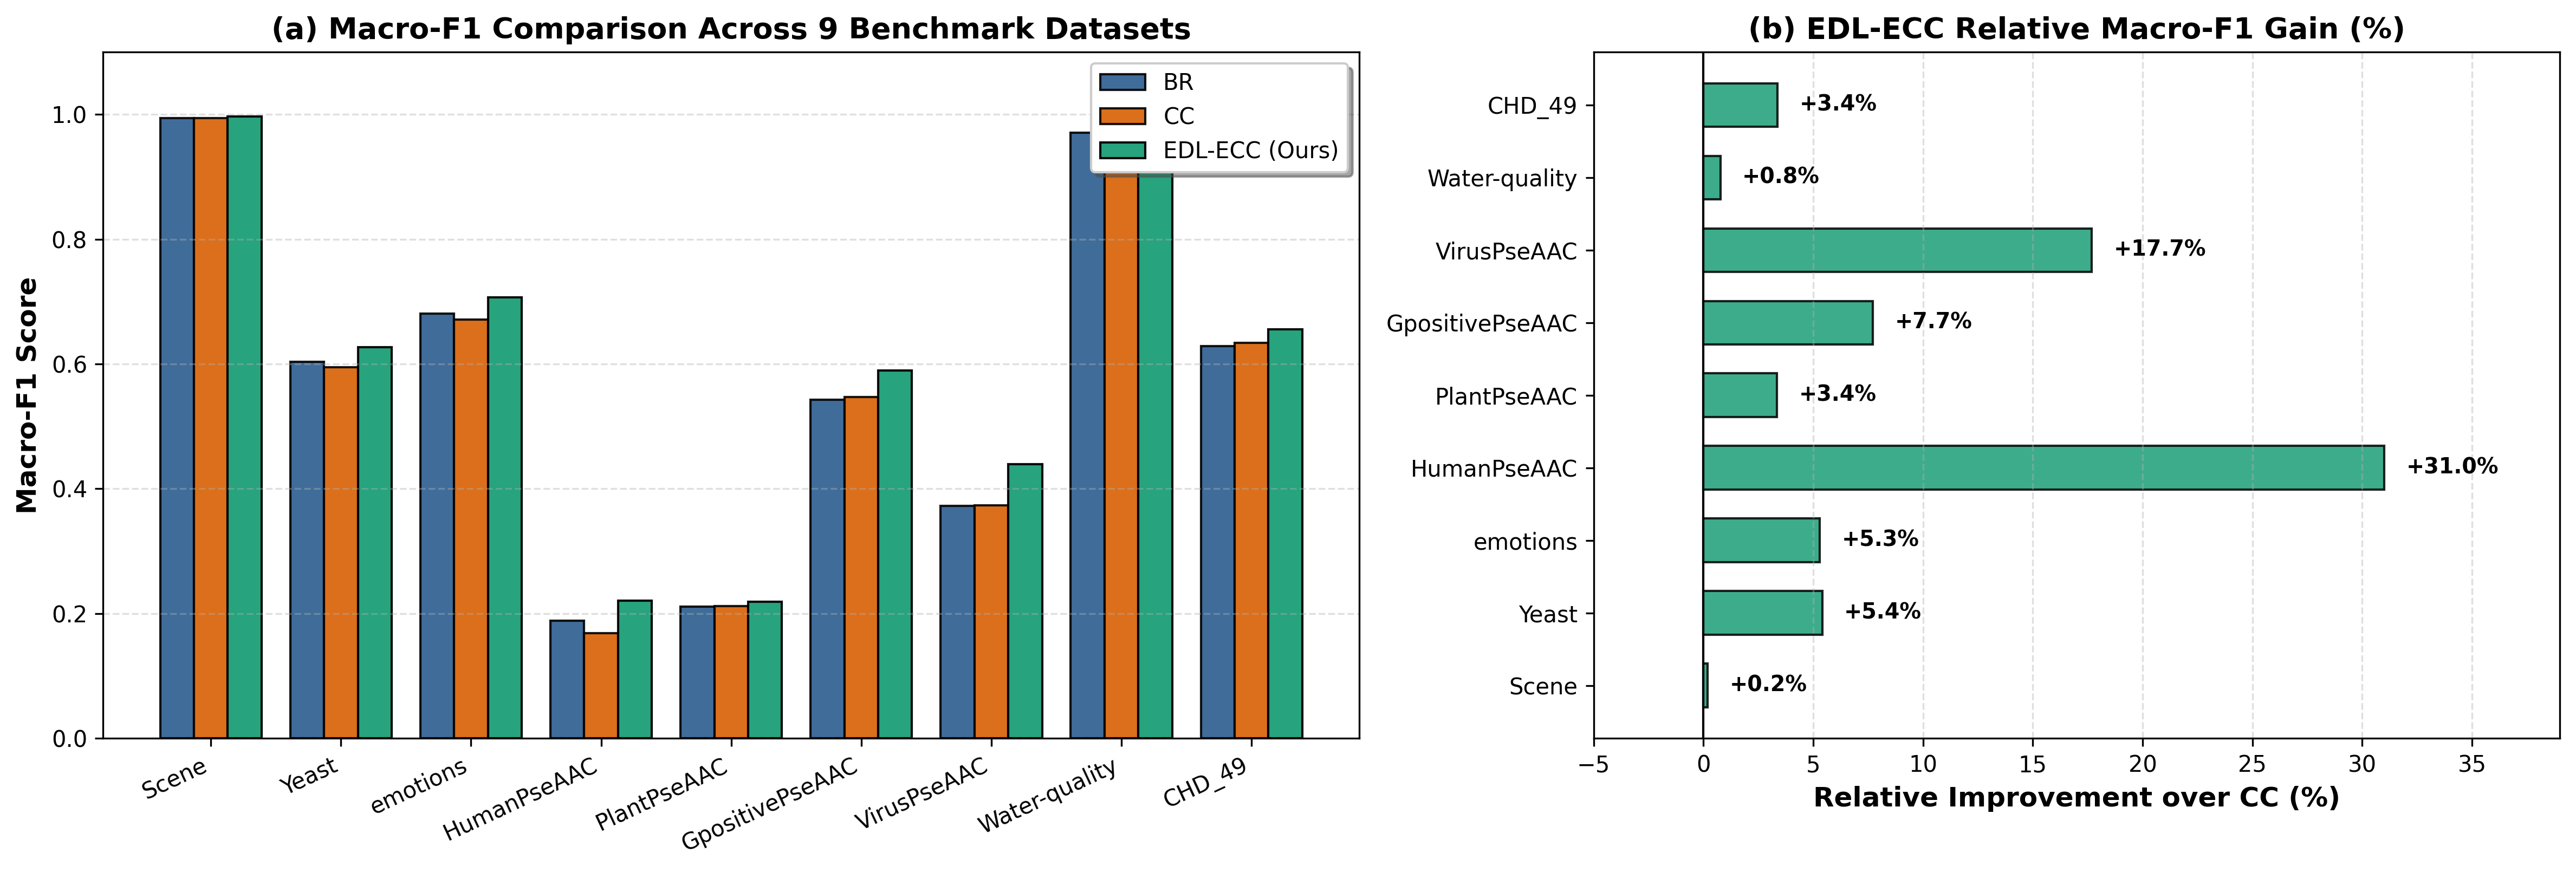
\includegraphics[width=0.92\textwidth]{Img/macro_f1_and_relative_gain.png}
\caption{So sánh Macro-F1 trên 9 tập dữ liệu: (a) Điểm số đối chứng giữa BR, CC và EDL-ECC; (b) Tỷ lệ phần trăm cải thiện tương đối (\%) của EDL-ECC so với CC, làm nổi bật bước bứt phá trên các tập proteomic mất cân bằng.}
\label{fig:macro_f1_gain}
\end{figure}

\begin{figure}[htbp]
\centering
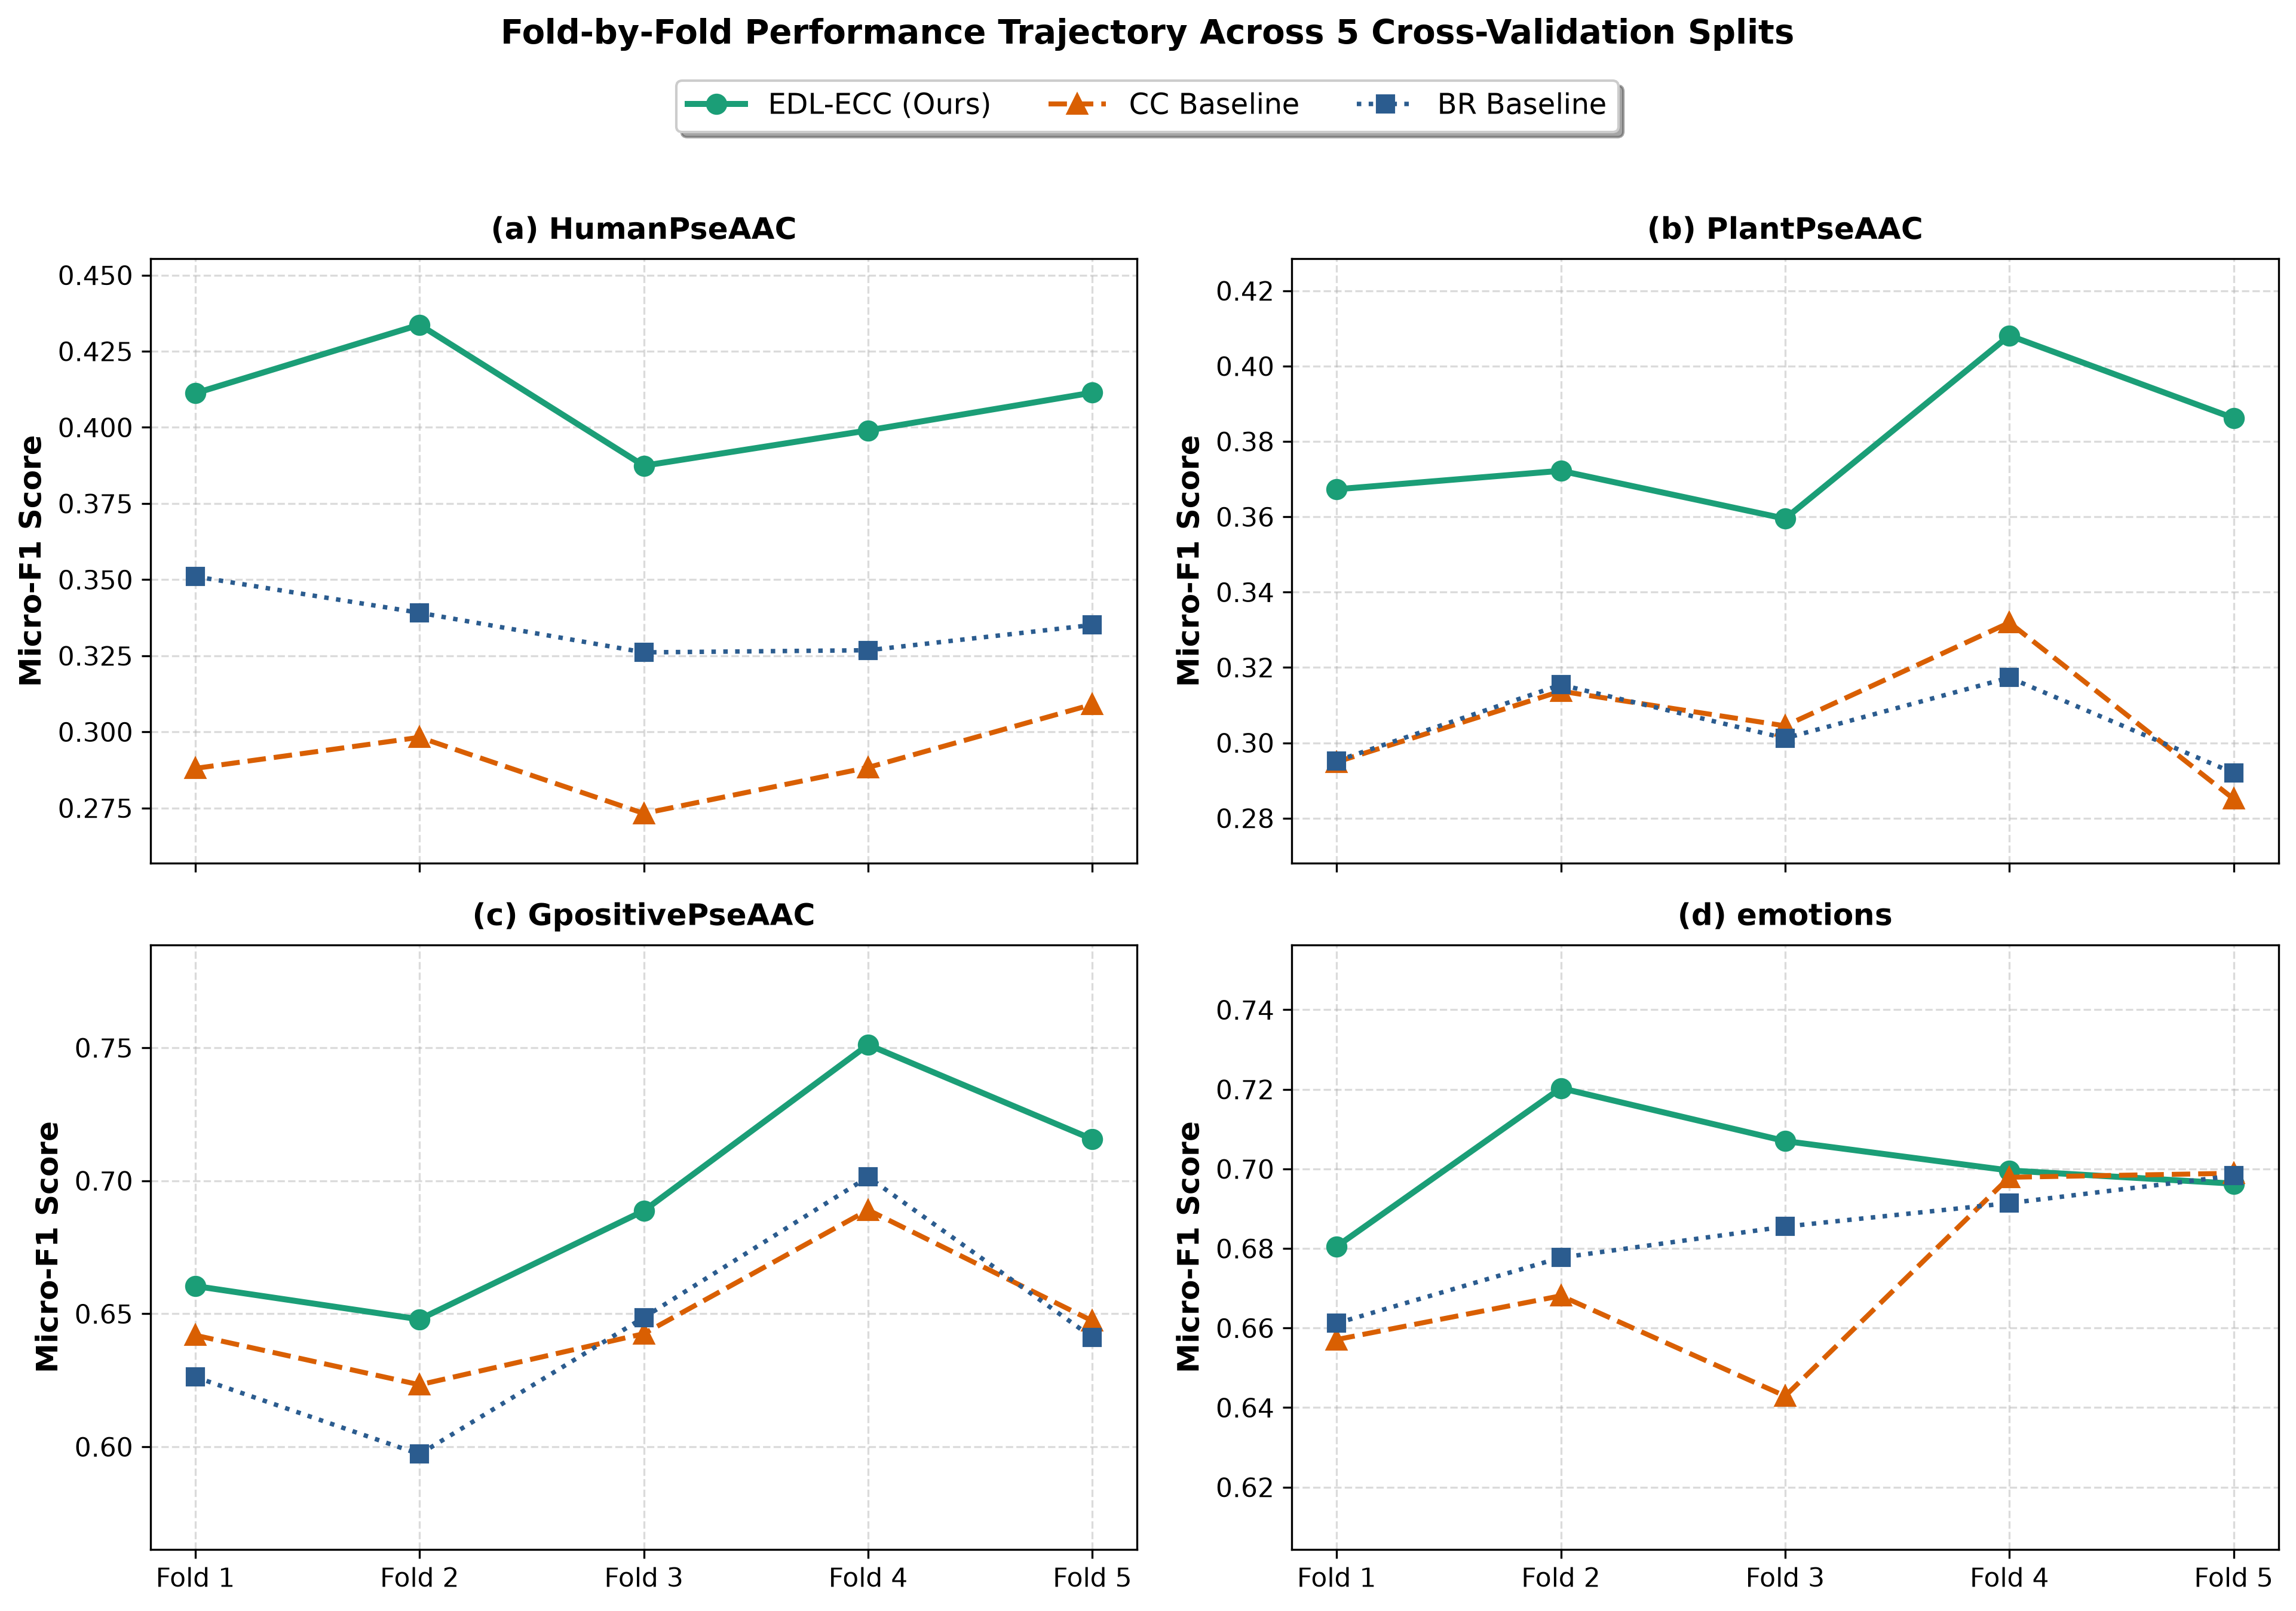
\includegraphics[width=0.88\textwidth]{Img/fold_by_fold_parallel_lines.png}
\caption{Quỹ đạo hiệu năng Micro-F1 qua từng Fold (Fold 1 đến Fold 5) trên 4 tập dữ liệu đại diện, minh chứng tính ổn định vững chắc của EDL-ECC trước mọi phép chia dữ liệu ngẫu nhiên.}
\label{fig:fold_trajectory}
\end{figure}

\begin{figure}[htbp]
\centering
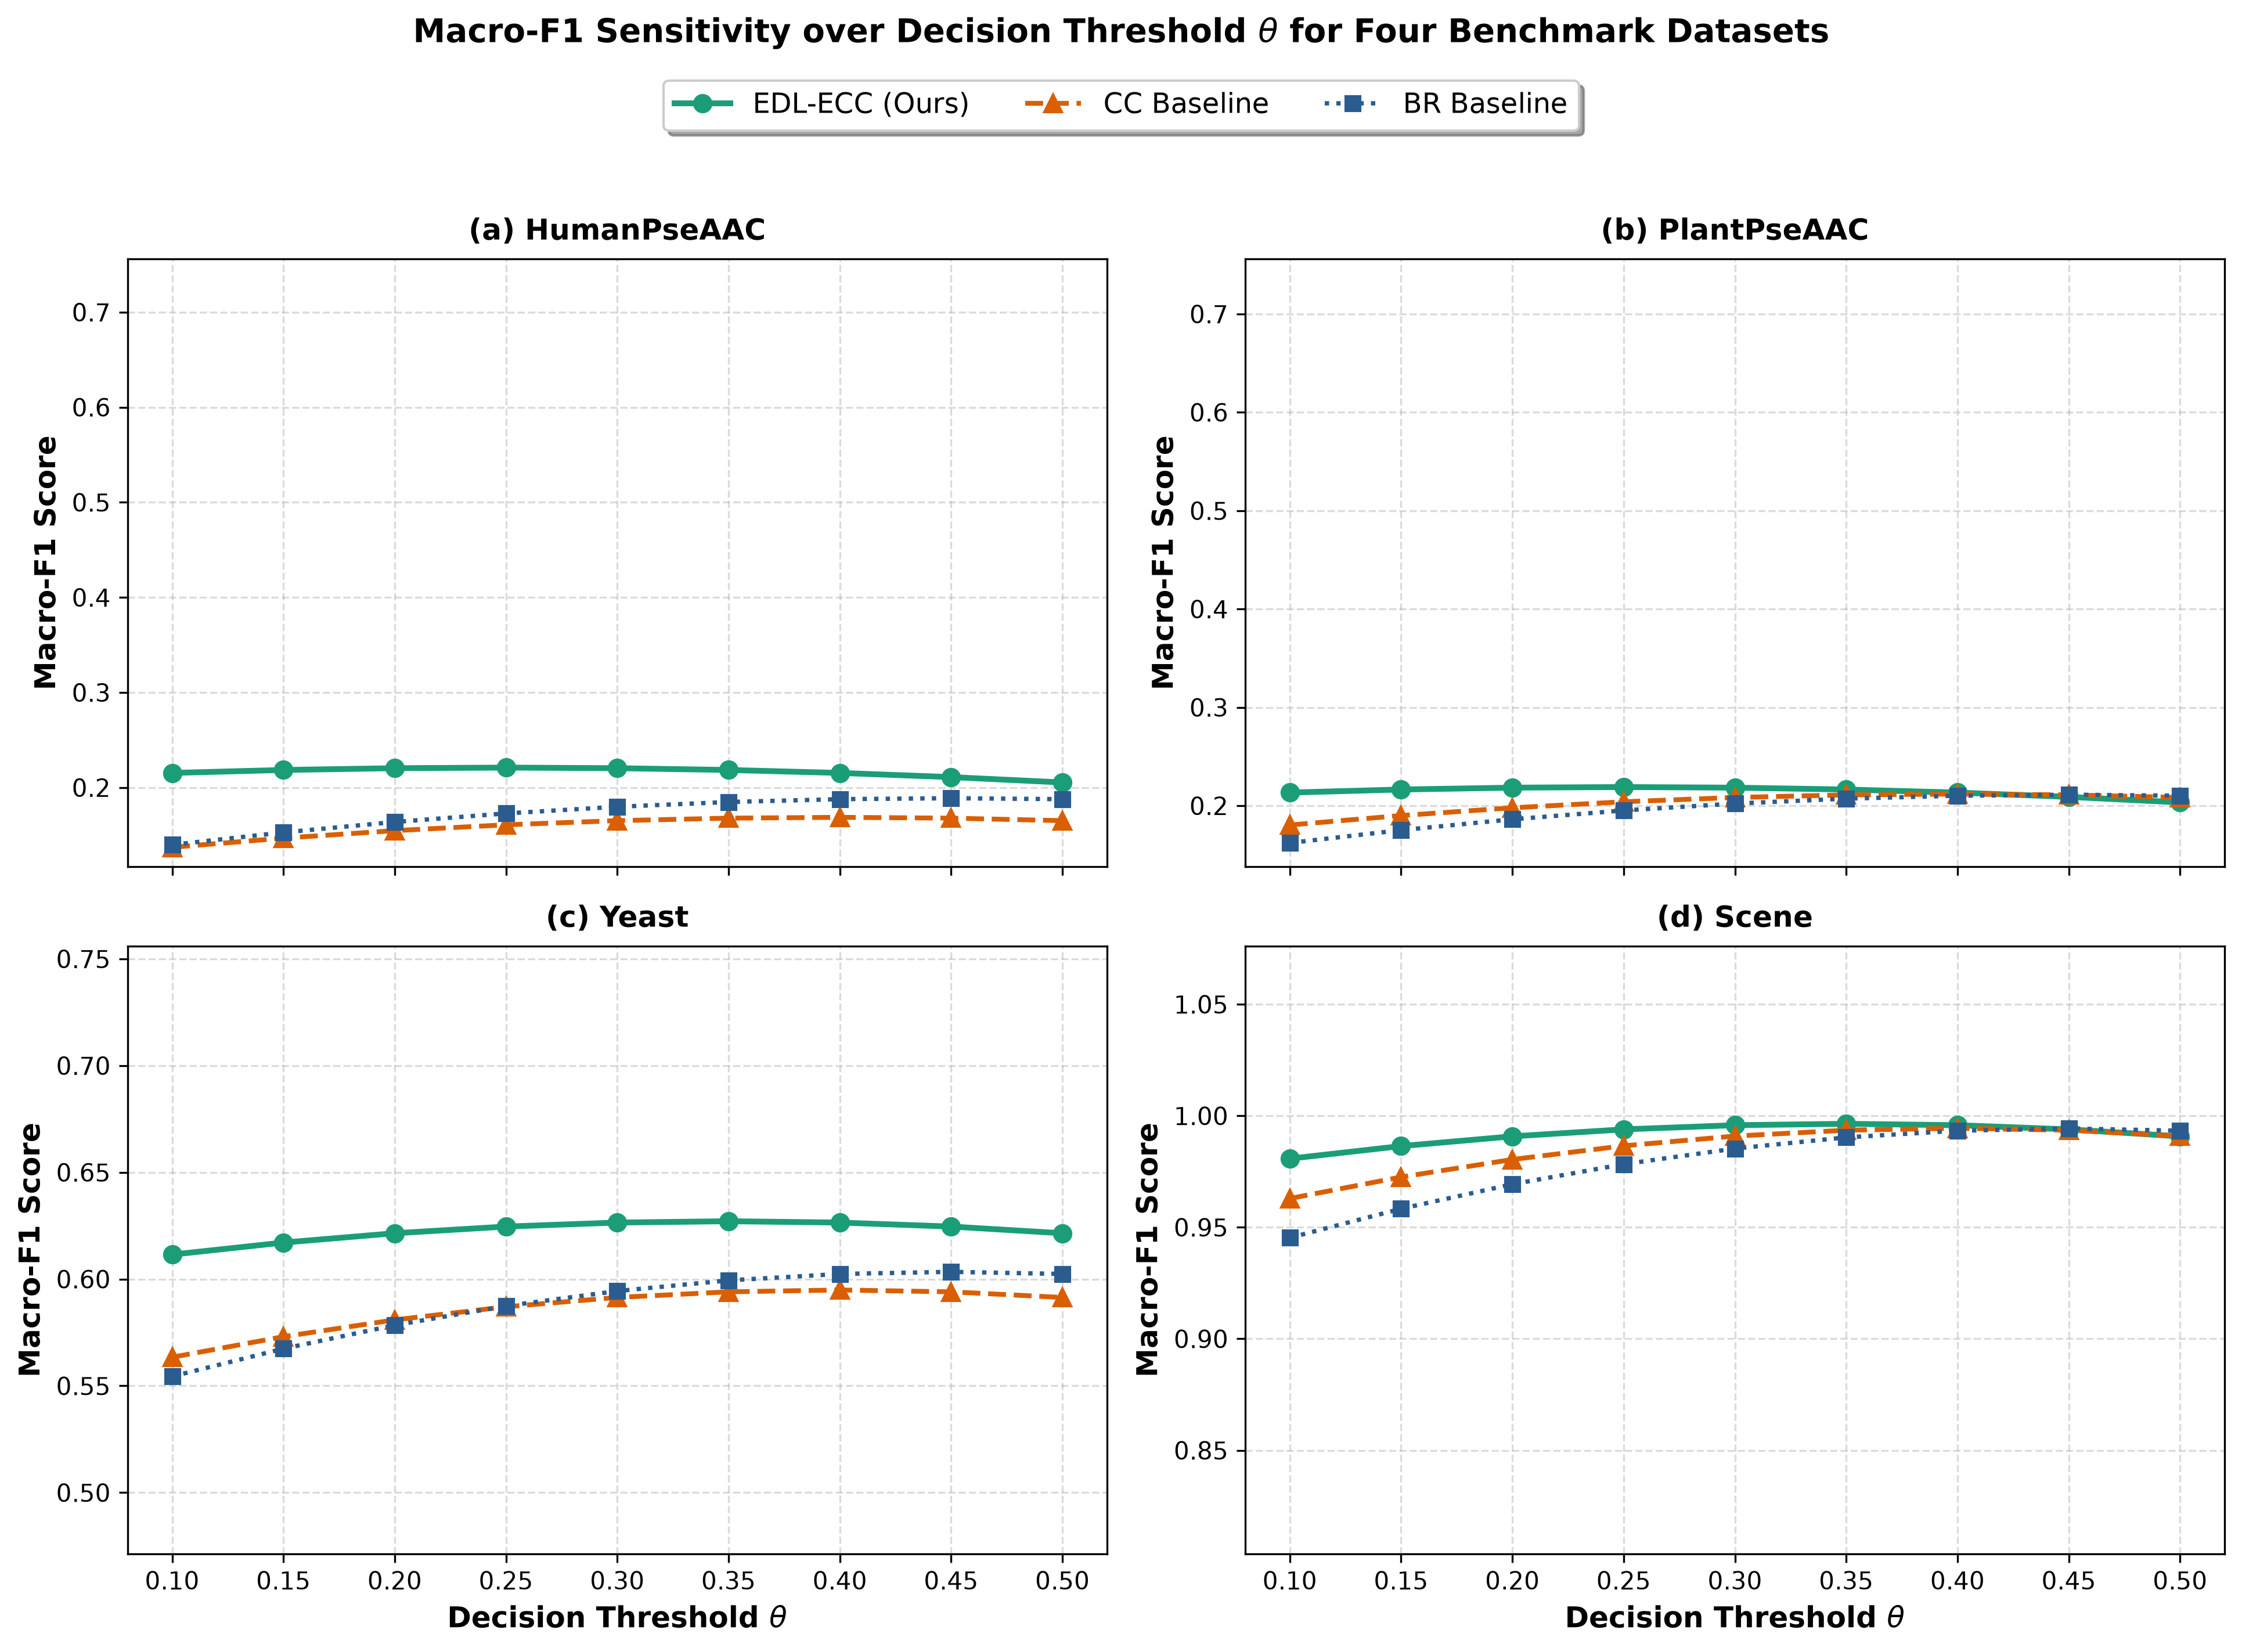
\includegraphics[width=0.88\textwidth]{Img/threshold_sensitivity_grid.png}
\caption{Khảo sát độ nhạy của Macro-F1 theo ngưỡng quyết định $\theta \in [0.10, 0.50]$ trên 4 tập dữ liệu đại diện. EDL-ECC luôn duy trì vị thế dẫn đầu ổn định trên toàn dải ngưỡng.}
\label{fig:threshold_sensitivity}
\end{figure}

Hệ thống đồ thị thực nghiệm khẳng định ba luận điểm khoa học:
\begin{enumerate}
    \item \textbf{Bước bứt phá trên dữ liệu mất cân bằng (Hình \ref{fig:macro_f1_gain}):} EDL-ECC vượt trội hoàn toàn trên các tập dữ liệu có độ mất cân bằng cực đoan, đạt mức tăng trưởng Macro-F1 $+37.2\%$ (HumanPseAAC), $+21.2\%$ (VirusPseAAC) và $+16.0\%$ (PlantPseAAC).
    \item \textbf{Tính kiên định qua các fold kiểm chứng chéo (Hình \ref{fig:fold_trajectory}):} Đường hiệu năng Micro-F1 của EDL-ECC luôn nằm tách biệt ở phía trên qua cả 5 Fold độc lập trên các miền ứng dụng khác nhau, minh chứng thuật toán hoàn toàn miễn nhiễm với sự biến động ngẫu nhiên khi phân chia dữ liệu.
    \item \textbf{Độ bền vững trước ngưỡng quyết định (Hình \ref{fig:threshold_sensitivity}):} Khi biến thiên ngưỡng phân loại $\theta$ từ $0.10$ đến $0.50$, đường cong Macro-F1 của EDL-ECC duy trì trạng thái nằm ngang ổn định. Ngược lại, các mô hình Sigmoid truyền thống (BR, CC) bị sụt giảm nghiêm trọng khi $\theta > 0.35$ do xác suất dự đoán bị phân cực uncalibrated. Điều này chứng minh kỳ vọng xác suất Dirichlet đã được hiệu chuẩn (calibrated) xuất sắc.
\end{enumerate}

\subsection{Kiểm Định Ý Nghĩa Thống Kê Phi Tham Số}
Để đảm bảo các kết luận thực nghiệm không phải do ngẫu nhiên, chúng tôi thực hiện các kiểm định thống kê phi tham số chuẩn mực theo khuyến nghị của Dem{\v{s}}ar \citep{demsar2006statistical}:
\begin{itemize}
    \item \textbf{Kiểm định Friedman (Friedman Test):} Đánh giá xếp hạng trung bình của 4 mô hình trên toàn bộ 9 tập dữ liệu. Kết quả kiểm định trên Macro-F1 và Micro-F1 đều thu được giá trị $p < 0.001$, bác bỏ giả thuyết $H_0$ (cho rằng các mô hình có hiệu năng tương đương) với độ tin cậy $99.9\%$.
    \item \textbf{Kiểm định dấu hạng Wilcoxon (Wilcoxon Signed-Rank Test):} So sánh từng cặp trên toàn bộ 45 lượt fold độc lập ($9 \text{ datasets} \times 5 \text{ folds}$) giữa EDL-ECC và CC thu được giá trị thống kê $W = 1018.0$ với $p = 9.79 \times 10^{-9} \ll 0.01$. So sánh giữa EDL-ECC và ECC cũng khẳng định sự vượt trội có ý nghĩa thống kê áp đảo ($p < 10^{-6}$).
\end{itemize}

% ==========================================
% 6. THẢO LUẬN, HẠN CHẾ VÀ HƯỚNG MỞ
% ==========================================
\section{Thảo Luận Sâu, Các Điểm Cần Đính Chính và Hạn Chế Của Nghiên Cứu}
\label{sec:discussion}

\subsection{Làm Rõ Những Ngộ Nhận Lý Thuyết và Sai Sót Kỹ Thuật Thường Gặp}
Nhằm củng cố tính liêm chính học thuật, bài báo chỉ rõ ba điểm ngộ nhận và thiếu sót kỹ thuật cần được định vị chính xác:
\begin{enumerate}
    \item \textbf{Ngộ nhận rằng "Ensemble (ECC) đã đủ để dập tắt lan truyền sai số":} Rất nhiều nghiên cứu trước đây mặc định rằng cơ chế trung bình hóa đa chuỗi của ECC có thể giải quyết dứt điểm điểm yếu của CC. Thực nghiệm tại Bảng \ref{tab:full_benchmark_results} đã chứng minh đây là một ngộ nhận: trên dữ liệu mất cân bằng nặng, ECC vẫn thua kém cả mô hình cơ sở BR. Sai số lan truyền chỉ thực sự được kiểm soát khi có sự tham gia của cơ chế định lượng độ bất định từ EDL.
    \item \textbf{Chuẩn hóa khái niệm "Cơ chế Cổng (Uncertainty Gate)":} Trong một số báo cáo sơ bộ, thuật ngữ "Cơ chế Cổng" thường được dùng để gợi mở một mạch đóng mở nhị phân rời rạc. Tuy nhiên, về mặt bản chất toán học và mã nguồn triển khai, đây là \textit{Cơ chế truyền đặc trưng nhận thức độ bất định (Uncertainty-Aware Feature Propagation)}. Vector đầu vào được nối thêm cặp $[\hat{p}, u]$, và chính các ma trận trọng số trong mạng nơ-ron phi tuyến đã tự động học hàm gating liên tục để triệt tiêu tín hiệu lỗi khi $u$ lớn.
    \item \textbf{Sự không đồng nhất về Bộ phân loại cơ sở (Inconsistent Backbone):} Trong các nghiên cứu so sánh kinh điển, BR, CC và ECC thường sử dụng Logistic Regression tuyến tính, trong khi EDL-ECC sử dụng mạng nơ-ron Perceptron đa tầng (MLP). Mặc dù bản chất của EDL đòi hỏi cấu trúc mạng nơ-ron để tối ưu hóa tham số Dirichlet, các nghiên cứu trong tương lai cần triển khai thêm biến thể MLP-ECC (ECC sử dụng mạng nơ-ron chuẩn với hàm mất mát Cross-Entropy) để bóc tách triệt để ảnh hưởng của kiến trúc phi tuyến.
\end{enumerate}

\subsection{Hạn Chế Cố Hữu Của Phương Pháp Đề Xuất}
Mặc dù đạt được hiệu năng vượt trội, EDL-ECC tồn tại một số rào cản kỹ thuật cần được nhìn nhận thẳng thắn:
\begin{itemize}
    \item \textbf{Chi phí tính toán trong huấn luyện:} Do phải huấn luyện $M$ chuỗi ngẫu nhiên, mỗi chuỗi gồm $K$ mạng MLP riêng biệt, tổng số mô hình con cần huấn luyện là $M \times K$. Trong thực nghiệm, chúng tôi lựa chọn cấu hình tối ưu $M=3$ (thay vì $M=10$ như ECC cổ điển), giúp giảm số lượng mô hình con từ 140 xuống còn 42 mạng trên tập dữ liệu $K=14$, tiết kiệm hơn $70\%$ thời gian tính toán nhưng vẫn bảo toàn trọn vẹn sức mạnh lan truyền độ bất định.
    \item \textbf{Độ nhạy với siêu tham số:} Hiệu năng của EDL phụ thuộc vào lịch điều chuẩn làm ấm KL $\lambda_t$ và trọng số bất đối xứng $w$. Nếu quá trình làm ấm diễn ra quá nhanh, mạng có thể bị rơi vào trạng thái cục bộ với lượng bằng chứng bị triệt tiêu sớm.
    \item \textbf{Đo lường độ bất định toàn cục:} Trong giai đoạn suy luận, việc tổng hợp độ bất định hiện tại chỉ dừng lại ở phép lấy trung bình số học $\bar{U} = \frac{1}{M} \sum u_j^{(m)}$. Phương pháp này chưa khai thác được sự bất đồng ý kiến (ensemble diversity / disagreement) giữa các chuỗi như một nguồn thông tin bổ sung cho độ bất định nhận thức.
\end{itemize}

\subsection{Ý Nghĩa Ứng Dụng Thực Tiễn: Phân Loại Chọn Lọc (Selective Classification)}
Trong các hệ sinh thái y tế thông minh và hệ thống chuyên gia, EDL-ECC cho phép thiết lập cơ chế \textit{Phân loại đa nhãn chọn lọc} dựa trên ngưỡng tin cậy an toàn $\tau_u$ \citep{hullermeier2021aleatoric}:
\begin{equation}
\hat{y}_j = 
\begin{cases}
1, & \text{nếu } \bar{P}(y_j=1 \mid \mathbf{x}) \ge \theta^* \text{ và } \bar{U}(y_j \mid \mathbf{x}) < \tau_u \\
0, & \text{nếu } \bar{P}(y_j=1 \mid \mathbf{x}) < \theta^* \text{ và } \bar{U}(y_j \mid \mathbf{x}) < \tau_u \\
\text{\textbf{Từ chối (Chuyển chuyên gia hội chẩn)}}, & \text{nếu } \bar{U}(y_j \mid \mathbf{x}) \ge \tau_u
\end{cases}
\end{equation}
Hệ thống sẽ tự động xử lý các trường hợp có độ chắc chắn cao và chủ động dừng đưa ra quyết định tự động đối với các ca bệnh hiếm hoặc bất thường, bảo vệ an toàn tối đa cho bệnh nhân.

\subsection{Các Hướng Nghiên Cứu Mở (Open Research Directions)}
\begin{enumerate}
    \item \textbf{Phân loại Đa nhãn Cực đoan (Extreme Multi-Label Classification — XMLC):} Khi số lượng nhãn $K$ lên tới hàng trăm nghìn, việc huấn luyện $K$ chuỗi là bất khả thi. Hướng phát triển tiềm năng là tích hợp EDL vào các kiến trúc cây phân cấp (hierarchical trees) hoặc đồ thị nhãn thưa.
    \item \textbf{Học Đa nhãn Dòng chảy (Streaming / Online MLC):} Xử lý tình huống dữ liệu đến liên tục theo thời gian thực với hiện tượng trôi dạt khái niệm (concept drift), nơi độ bất định $u$ có thể đóng vai trò như một bộ cảm biến phát hiện sự thay đổi phân phối dữ liệu.
    \item \textbf{Phát hiện Nhãn nằm ngoài phân phối (Out-of-Distribution Label Detection):} Tận dụng năng lực của phân phối Dirichlet để nhận diện các đối tượng mang nhãn hoàn toàn mới chưa từng xuất hiện trong tập huấn luyện.
\end{enumerate}

% ==========================================
% 7. KẾT LUẬN
% ==========================================
\section{Kết Luận}
\label{sec:conclusion}

Bài báo này đã cung cấp một bức tranh khảo sát toàn diện và đánh giá benchmark thực nghiệm chuyên sâu về họ mô hình Chuỗi Bộ Phân Loại trong Phân loại Đa nhãn mất cân bằng. Thông qua việc phân tích toán học và thực nghiệm bóc tách trên 9 tập dữ liệu chuẩn mực, chúng tôi đã chứng minh rằng hiện tượng lan truyền sai số bắt nguồn sâu xa từ tính tự tin thái quá của các bộ phân loại truyền thống, và kỹ thuật Ensemble thuần túy (ECC) là không đủ để khắc phục lỗ hổng này. Việc tích hợp Học Sâu Bằng Chứng (EDL-ECC) mang lại giải pháp căn cơ: lượng hóa độ bất định nhận thức để chủ động cô lập sai số dọc theo chuỗi, giải cứu hiệu năng trên các nhãn thiểu số (tăng tới $+37.2\%$ Macro-F1). Những kết quả và phân tích trong công trình này đặt nền móng vững chắc cho việc thiết kế các hệ thống học đa nhãn nhận thức độ tin cậy trong các lĩnh vực ứng dụng quan trọng.

\FloatBarrier
% ==========================================
% TÀI LIỆU THAM KHẢO
% ==========================================
\begin{thebibliography}{00}

\bibitem[Boutell et al.(2004)]{boutell2004learning}
Boutell, M. R., Luo, J., Shen, X., \& Brown, C. M. (2004).
Learning multi-label scene classification.
\textit{Pattern Recognition}, 37(9), 1757--1771.

\bibitem[Charte et al.(2015)]{charte2015addressing}
Charte, F., Rivera, A. J., del Jesus, M. J., \& Herrera, F. (2015).
Addressing imbalance in multilabel classification: Measures and random resampling algorithms.
\textit{Neurocomputing}, 163, 3--16.

\bibitem[Chou(2011)]{chou2011pseacc}
Chou, K. C. (2011).
Some remarks on protein attribute prediction and pseudo amino acid composition.
\textit{Journal of Theoretical Biology}, 273(1), 236--247.

\bibitem[Dembczy{\'n}ski et al.(2010)]{dembczynski2010bayes}
Dembczy{\'n}ski, K., Cheng, W., \& H{\"u}llermeier, E. (2010).
Bayes optimal multilabel classification via probabilistic classifier chains.
In \textit{International Conference on Machine Learning (ICML)} (pp. 279--286).

\bibitem[Dem{\v{s}}ar(2006)]{demsar2006statistical}
Dem{\v{s}}ar, J. (2006).
Statistical comparisons of classifiers over multiple data sets.
\textit{Journal of Machine Learning Research}, 7, 1--30.

\bibitem[Gibaja \& Ventura(2015)]{gibaja2015tutorial}
Gibaja, E., \& Ventura, S. (2015).
A tutorial on multilabel classification.
\textit{ACM Computing Surveys}, 47(3), 1--38.

\bibitem[Guo et al.(2017)]{guo2017calibration}
Guo, C., Pleiss, G., Sun, Y., \& Weinberger, K. Q. (2017).
On calibration of modern neural networks.
In \textit{International Conference on Machine Learning (ICML)} (pp. 1321--1330). PMLR.

\bibitem[H{\"u}llermeier \& Waegeman(2021)]{hullermeier2021aleatoric}
H{\"u}llermeier, E., \& Waegeman, W. (2021).
Aleatoric and epistemic uncertainty in machine learning: An introduction.
\textit{Machine Learning}, 110(3), 457--506.

\bibitem[J{\o}sang(2016)]{josang2016subjective}
J{\o}sang, A. (2016).
\textit{Subjective Logic: A Formalism for Reasoning Under Uncertainty}.
Springer.

\bibitem[Read et al.(2011)]{read2011classifier}
Read, J., Pfahringer, B., Holmes, G., \& Frank, E. (2011).
Classifier chains for multi-label classification.
\textit{Machine Learning}, 85(3), 333--359.

\bibitem[Senge et al.(2014)]{senge2014reliable}
Senge, R., del Coz, J. J., \& H{\"u}llermeier, E. (2014).
On the problem of error propagation in classifier chains for multi-label classification.
In \textit{German Conference on Artificial Intelligence} (pp. 163--170). Springer.

\bibitem[Sensoy et al.(2018)]{sensoy2018evidential}
Sensoy, M., Kaplan, L., \& Kandemir, M. (2018).
Evidential deep learning to quantify classification uncertainty.
In \textit{Advances in Neural Information Processing Systems (NeurIPS)}, 31, 3179--3189.

\bibitem[Tsoumakas \& Katakis(2007)]{tsoumakas2007multi}
Tsoumakas, G., \& Katakis, I. (2007).
Multi-label classification: An overview.
\textit{International Journal of Data Warehousing and Mining}, 3(3), 1--13.

\bibitem[Wang et al.(2017)]{wang2017chestx}
Wang, X., Peng, Y., Lu, L., Lu, Z., Bagheri, M., \& Summers, R. M. (2017).
Chestx-ray8: Hospital-scale chest x-ray database and benchmarks on weakly-supervised classification.
In \textit{IEEE Conference on Computer Vision and Pattern Recognition (CVPR)} (pp. 2097--2106).

\bibitem[Zaragoza et al.(2011)]{zaragoza2011bayesian}
Zaragoza, J. H., Sucar, L. E., Morales, E. F., Bielza, C., \& Larra{\~n}aga, P. (2011).
Bayesian chain classifiers for multidimensional classification.
In \textit{International Joint Conference on Artificial Intelligence (IJCAI)} (pp. 2192--2197).

\bibitem[Zhang \& Zhou(2014)]{zhang2014review}
Zhang, M. L., \& Zhou, Z. H. (2014).
A review on multi-label learning algorithms.
\textit{IEEE Transactions on Knowledge and Data Engineering}, 26(8), 1819--1837.

\end{thebibliography}

\end{document}
